\chapter{Situação atual}
Com o aumento da capacidade de passageiros e carga e a 
necessidade de uma maior 
segurança, começou a se fazer necessário trazer ao cockpit vários
documentos como checklist de procedimentos; log book; cartas de 
navegação, de saída, de aproximação, do aeródromo; tabelas de 
performance da aeronave etc. 

Para levar tudo isto costumava-se usar uma maleta (a Flight Bag),
obviamente esta ficava muito pesada.

Com a miniaturização dos computadores e surgimentos dos tablets, 
começaram a ser desenvolvidos programas que substituíam partes
ou todos estes documentos, é a chamada maleta de voo eletrônica,
mais conhecida pela sigla em Inglês EFB (\textit{Electronic Flight Bag}).

Nos simuladores de voo para computador pessoal, algumas aeronaves
simulam este equipamento como o Airbus A320neo desenvolvido pela
\textit{FlyByWire Simulations}. Apesar de ser uma aeronave \textit{freeware}, ela 
é bem sofisticada chegando ao nível de realismo da \textit{Fenix Simulations}
ou da \textit{ToLiss Simulations}, duas produtoras com modelos pagos do A320.

\begin{figure}[ht]
    \begin{center}
    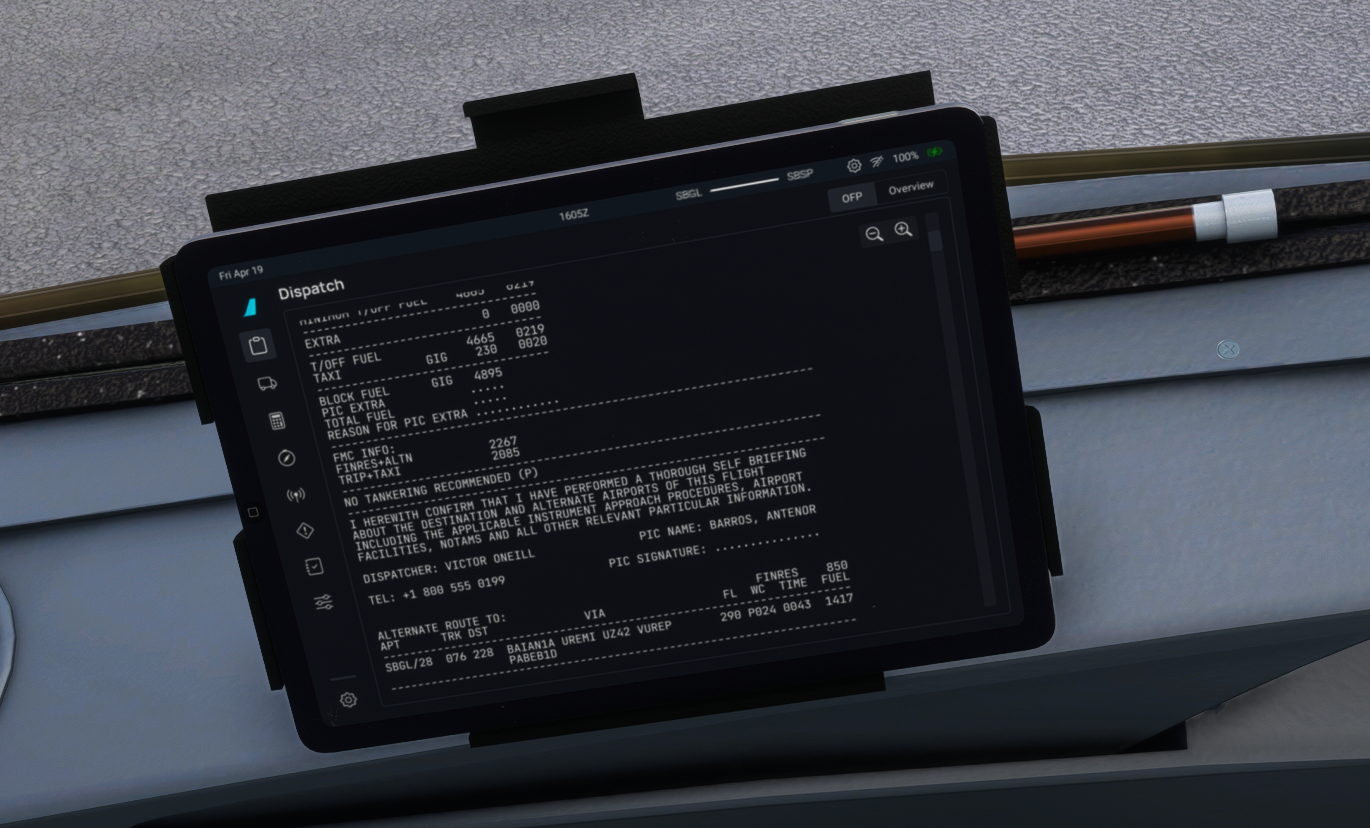
\includegraphics[width=400pt]{img/efb-a320.png}
    \caption{Exemplo de um EFB no Flight Simulator 2020 na aeronave A320neo}
    \label{fig:efb-a320}
    \end{center}
\end{figure}

Contudo, o METAR do aeródromo não se encontra disponível no EFB.
É possível usar o computador de bordo da aeronave (FMC) e conseguir
esta informação. Também é possível sintonizar na frequência do ATIS,
mas isto só funcionará se o avião já estiver perto do aeródromo.

O que muitos jogadores fazem é acessar o AISWEB (\url{https://aisweb.decea.mil.br/}) , sistema oficial brasileiro
de informações aeronáuticas. 

\begin{figure}[ht]
    \begin{center}
    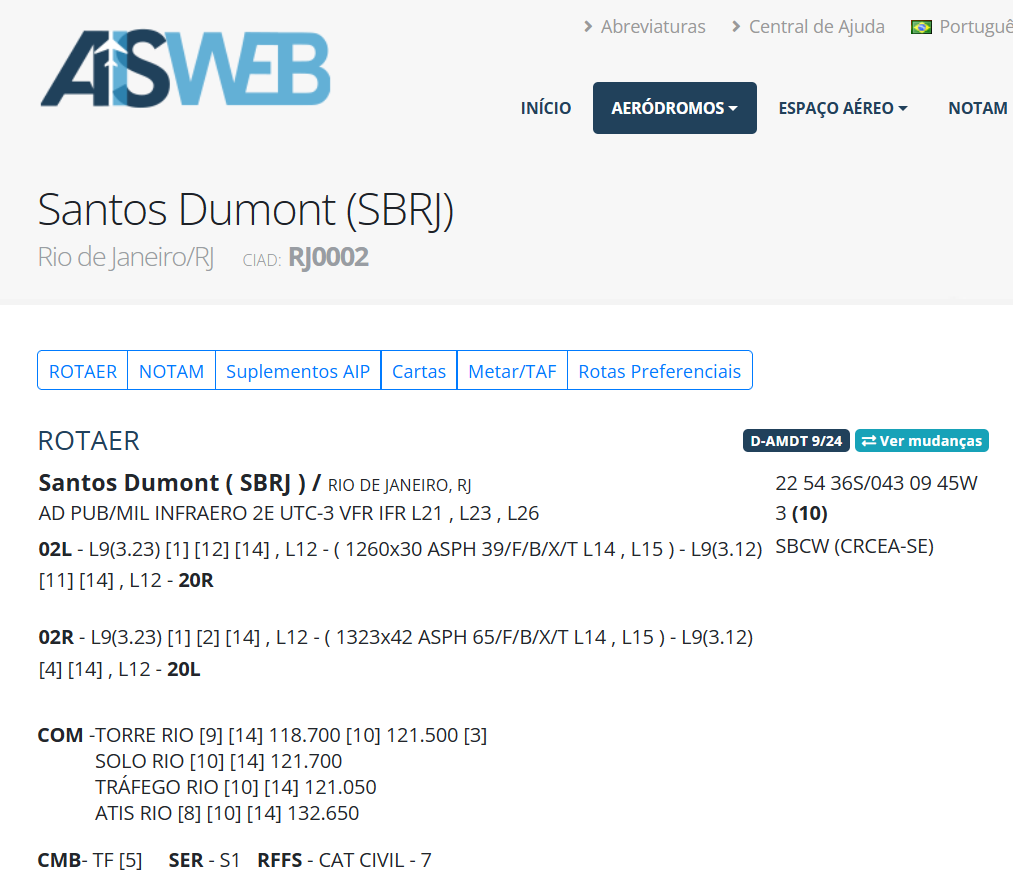
\includegraphics[width=400pt]{img/aisweb.png}
    \caption{AISWEB com informações de pista, frequências de comunicação e navegação para o Santos Dumont}
    \label{fig:aisweb}
    \end{center}
\end{figure}

É um site extremamente completo, podendo
ser usado em operações reais, mas para o jogador iniciante seria 
de valia uma interface mais simples.

O AISWEB exibe o METAR no aeroporto, mas não explica para o que cada campo serve.

\begin{figure}[ht]
    \begin{center}
    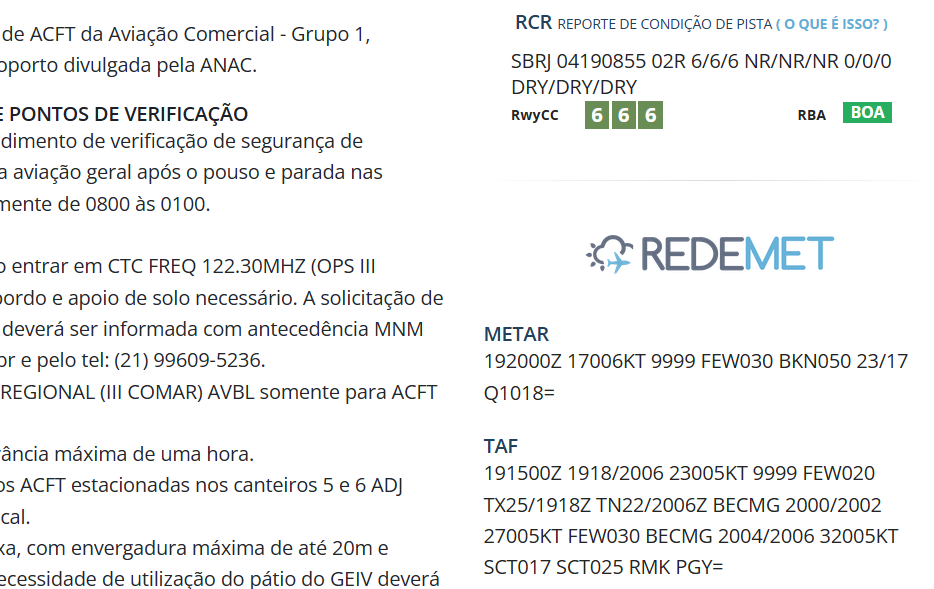
\includegraphics[width=400pt]{img/metar-aisweb.png}
    \caption{METAR do Santos Dumont no AISWEB}
    \label{fig:aisweb}
    \end{center}
\end{figure}

O site METAR-TAF (\url{https://metar-taf.com/}) é o decoder mais conhecido, possui uma interface 
gráfica bem construída
e muito fácil de entender, mas não possui a lista de frequência dos aeroportos e
de radionavegação.

\begin{figure}[ht]
    \begin{center}
    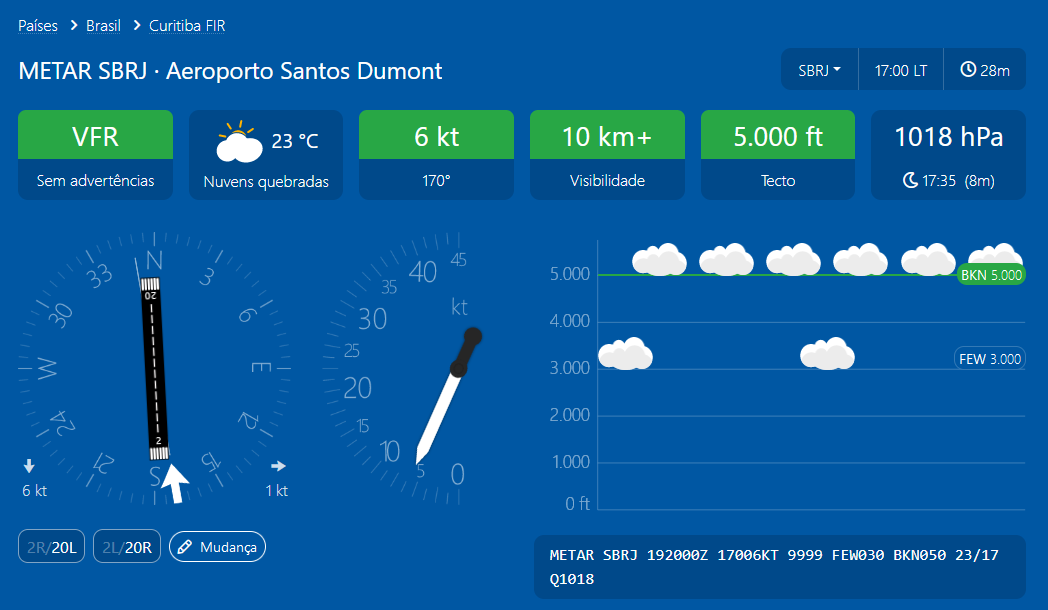
\includegraphics[width=400pt]{img/ui-metar-taf.png}
    \caption{Interface gráfica do METAR-TAF}
    \label{fig:metar-taf}
    \end{center}
\end{figure}
